\documentclass[xcolor=pdftex,dvipsnames,table,final]{beamer}
\mode<presentation>
{
  \usetheme{PosterCERG}
}
% size in width and height is in cm
% Arch D: 24"x36" use 60.96 x 91.44 Typical size for our printer, use 3 columns, scale=0.8 to fit more text
% each column should be 0.3\linewidth
% Arch E: 36"x48" use 91.44 x 121.92 OK for FedexKinko, use 4 columns
% each column should be 0.22\linewidth
\usepackage[orientation=portrait,size=custom,width=76.2,height=106.68,scale=1]{beamerposter}
% DATE-2016 Poster format
% DIN-A0-Portrait ----1189mm X 841mm or 118.9cm x 84.1cm or 46.8in x 33.1in 
%\usepackage[orientation=portrait, size=custom, width=84.1, height=118.9 scale=1.0]{beamerposter}sd
\usepackage{multirow,wrapfig}
\usepackage[labelformat=empty,justification=centering]{caption}
\usepackage{tikz}
\usepackage{lmodern}
\usepackage{multirow}
\usepackage{listings}
\usetikzlibrary{fit,arrows,calc,positioning}
%\usepackage{wrapfig}
%%%%%%%%%%% Additional packages-Panci
\usepackage[T1]{fontenc}

\definecolor{ocean}{RGB}{0,205,255}
\definecolor{beamerbackground}{rgb}{0.5,0.5,0.3}
\newcommand{\rb}[1]{\raisebox{1.3ex}[-1.3ex]{#1}}
\newcommand{\thb}[1]{\multicolumn{1}{c}{\textbf{#1}}}
\newcommand{\thbr}[1]{\multicolumn{1}{c|}{\textbf{#1}}}

\newcommand{\urlwofont}[1] { \urlstyle{same}\url{#1} }
     
\graphicspath{{figures/}}
\title{\LARGE eXtended eXternal Benchmarking eXtension\\ \vspace{0.5ex}(XXBX)}
\author{Matthew R. Carter \and Raghurama R. Velegala \and Snehal Patil \and John Pham \and Jens-Peter Kaps}%\vspace{-2ex}
\institute{\vspace{-1ex}Department of Electrical and Computer Engineering, George Mason University, Fairfax, Virginia 22030, USA }
\date{March}

\begin{document}
\lstset{%
  basicstyle=\ttfamily,
  language=bash,
  commentstyle=\color{tabutter},
  keywordstyle=\color{black},
  numberstyle=\color{cergbg1},
  stringstyle=\color{ta3orange},
  identifierstyle=\color{cergbg1}
}
\begin{frame}[fragile]{} 
  \begin{columns}[t, totalwidth=\textwidth]
% ---------------------------------------------------------------------------
%   FIRST COLUMN
% ---------------------------------------------------------------------------
    \begin{column}{.31\linewidth}

% ---------------------------------------------------------------------------
      \begin{block}{Abstract}
Many cryptographic standards are determined through competitions in which 
candidate algorithms are evaluated for their security and performance in software as
well as in hardware. 
The latest such competition is the Lightweight Cryptography Standardization
Process by NIST. 
%The submission requirements published in April 2018 call for
%Authenticated Encryption with Associated Data (AEAD) and hash function algorithms.
%This competition
It targets in particular resource-constrained devices such as 
microcontrollers.
%
The eXtended eXternal Benchmarking eXtension (XXBX) is a tool for benchmarking the performance, 
memory usage, and power / energy consumption of cryptographic software on microcontrollers. 
It is an extension to the System for Unified Performance Evaluation Related to Cryptographic 
Operations and Primitives (SUPERCOP) which benchmarks a large variety of cryptographic primitives 
on general purpose computers. XXBX extends it in the sense that it allows for benchmarking on 
embedded platforms and adds metrics for RAM and ROM usage as well as power / energy consumption. 
      \end{block}

% ---------------------------------------------------------------------------
      \begin{block}{Motivation}
        \begin{itemize}
          \item The move to the Internet of Things (IoT) leads to formerly 
                ``dumb'' devices being connected to the Internet.
          \item They require some level of security $\Rightarrow$ cryptographic algorithms.
          \item IoT promises a dramatic increase in devices, many will be microcontrollers or System on Chips (SOCs).
          \item 32-bit microcontrollers are projected to take lead over 8/16-bit.% by 2018.
          \item 51\% of all 32-bit microcontrollers were ARM based in 2012.
        \end{itemize}
        \begin{center}
          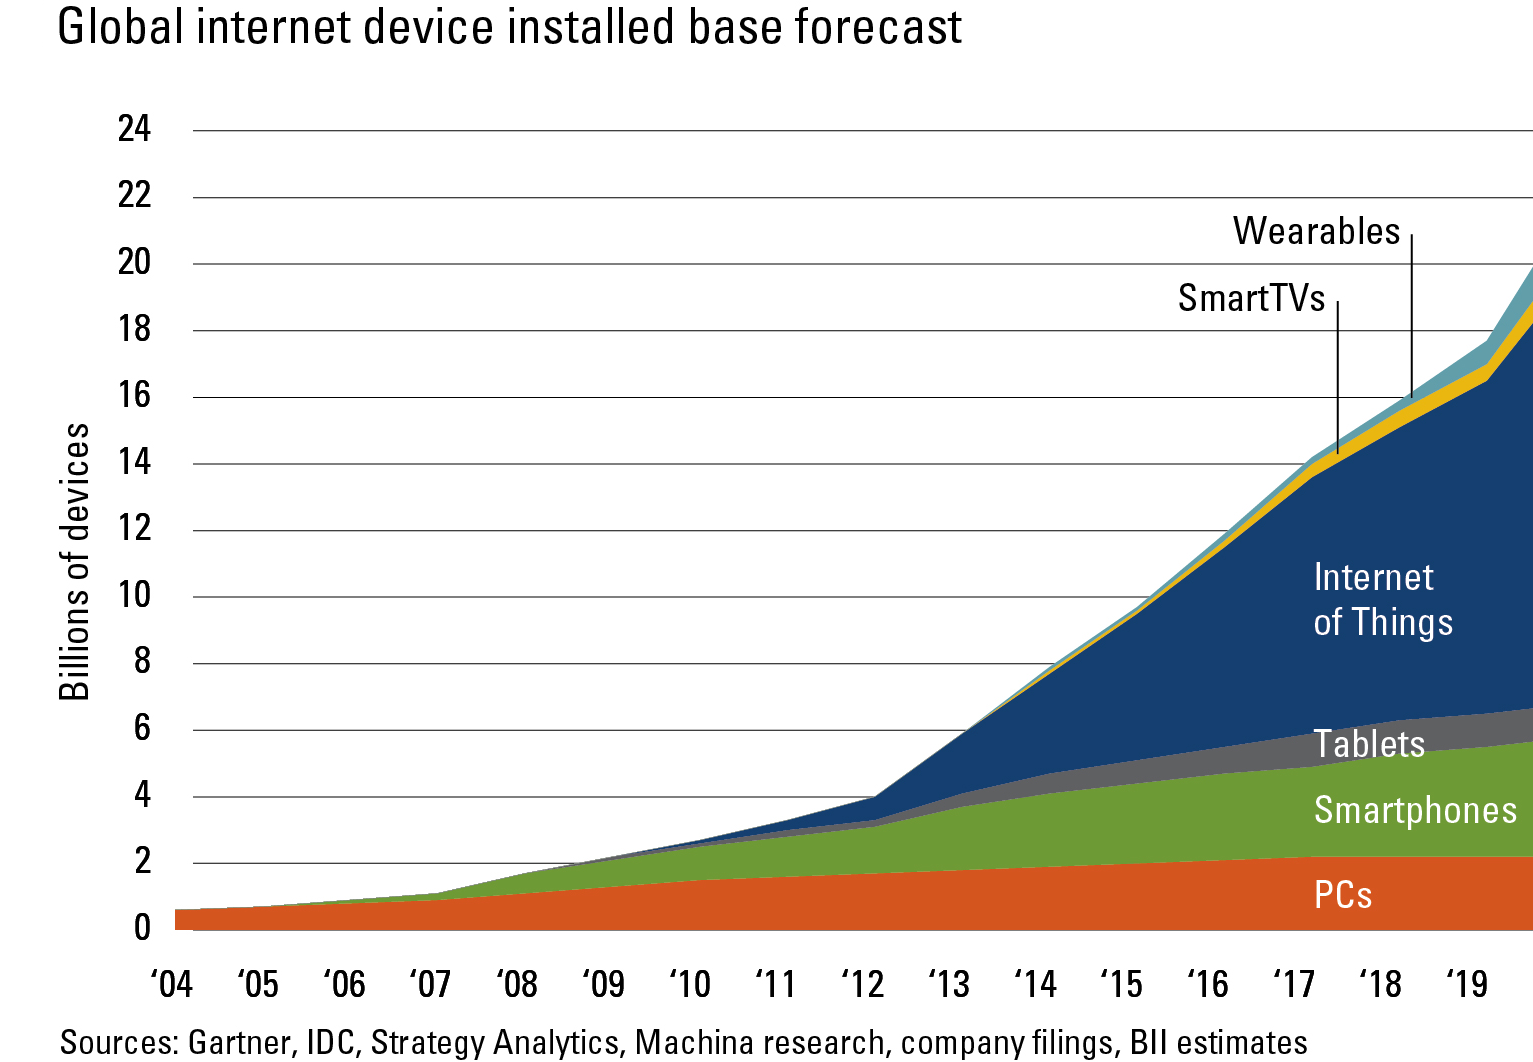
\includegraphics[scale=1.0]{figures/IMS-Internet_of_things.png}
      
          \vspace{-1ex}
          {\tiny \copyright 2015 AlixPartners, LLP}
        \end{center}
      \end{block}
	 
%---------------------------------------------------------------------------------
      \begin{block}{Benchmarking Tools}
        \begin{itemize}
          \item SUPERCOP
            \begin{itemize}
              \item System for Unified Performance Evaluation Related to Cryptographic Operations and Primitives
              \item Benchmarks many implementations of many primitives across multiple
                  operations on multiple hardware platforms.
              \item Supports environments capable of running Linux and hosting a
                  compiler.
              \item Series of shell scripts and C test harnesses, and comprehensive
                  collection of algorithm primitive implementations.
              \item Verifies correct execution of implementations and times cycles
                  required per byte processed.
%              \item Does not measure ROM and RAM usage or power consumption.
              \begin{center}
                  \url{http://bench.cr.yp.to/supercop.html}
              \end{center}
            \end{itemize}
        \end{itemize}
        \begin{center}
        \begin{minipage}[t]{0.9\linewidth}  
        \setbeamercolor{padding}{fg=white, bg=cergbg1}
        \begin{beamercolorbox}[rounded=true]{padding}
          \textbf{Missing Features}\small
          \begin{itemize}
            \item Does not measure ROM usage, RAM usage, power consumption.
            \item Does not support cross-compilation.
            \item Does not support microcontrollers.
          \end{itemize}
        \end{beamercolorbox}
        \end{minipage}
        \end{center}
        \begin{itemize}
          \item XBX
            \begin{itemize}
              \item eXternal Benchmarking eXtension (XBX) to SUPERCOP
              \item Automated testing on real microcontrollers.
              \item Compatibility with SUPERCOP algorithm collection (``algopacks'') and output format.
              \item Low cost hardware and software.
              \item Our contribution to original XBX was to port it to the MSP430
                  platform and provide results for SHA-3 finalists..
              \item Measures ROM and RAM usage. %Does not measure power consumption.
            \end{itemize}
        \end{itemize}
        \begin{center}
        \begin{minipage}[t]{0.9\linewidth}  
        \setbeamercolor{padding}{fg=white, bg=cergbg1}
        \begin{beamercolorbox}[rounded=true]{padding}
          \textbf{Missing Features}\small
          \begin{itemize}
            \item Does not measure power consumption.
            \item Harness device (ATmega32) limits future expansion.
          \end{itemize}
        \end{beamercolorbox}
        \end{minipage}
        \end{center}

      \end{block}
%-----------------------------------------------------------------------------------
%      \begin{block}{Metrics}
%        {\large\textbf{Throughput}}
%        \begin{itemize}
%          \item Measured in cycles per byte
%        \end{itemize}
%        {\large\textbf{RAM Usage}}
%        \begin{itemize}
%          \item Item 
%        \end{itemize}
%        {\large\textbf{ROM Usage}}
%        \begin{itemize}
%          \item Item 
%        \end{itemize}
%        {\large\textbf{Power Consumption}}
%        \begin{itemize}
%          \item Item 
%        \end{itemize}
%      \end{block}
%        
% ---------------------------------------------------------------------------
      \begin{block}{XXBX}
        {e\color{red}X}tended e{\color{red}X}ternal {\color{red}B}enchmarking 
        e{\color{red}X}tention extends the XBX by:% 
        \begin{itemize}
          \item Support for power and energy measurement.
          \item Support for Authenticated Encryption with Associated Data (AEAD) and hash functions
                to support NIST Lightweight Cryptography competition.
          \item Usage of a new harness with a powerful microcontroller running FreeRTOS.
          \item Rewritten software in Python 3 (was bash and perl).
          \item Storage of results in SQLite database.
        \end{itemize}
        \begin{center}
          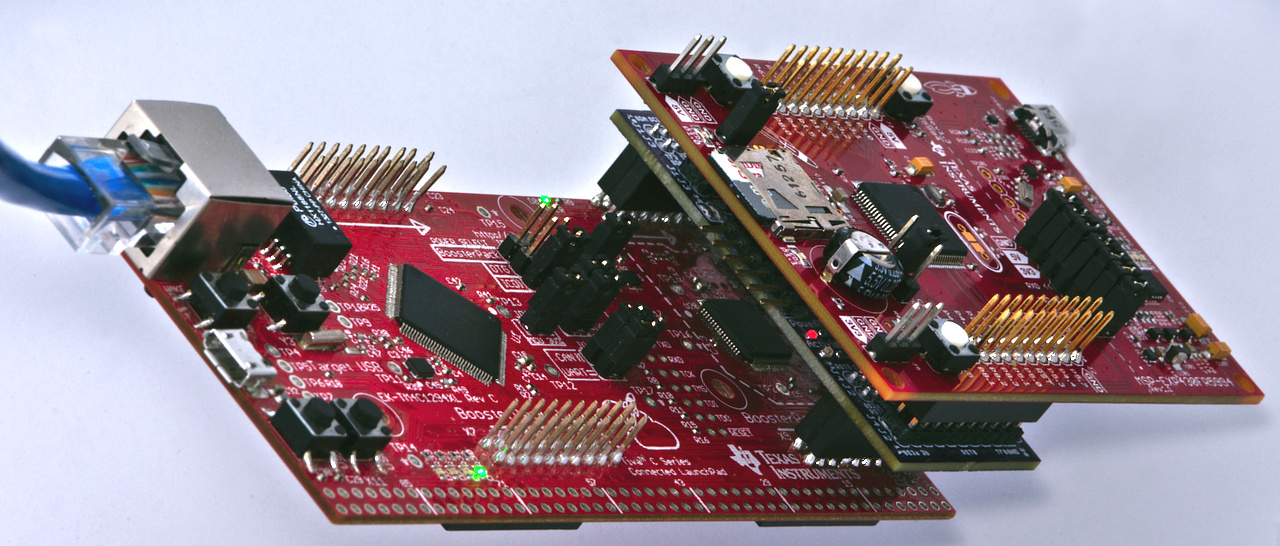
\includegraphics[scale=1.5]{../figures/xxbx-tilted}
        \end{center} 
      \end{block}
%---------------------------------------------------------------------------------
    \end{column}
% ---------------------------------------------------------------------------
\begin{column}{.675\linewidth}
   \begin{columns}%[t]
%   SECOND COLUMN
% ---------------------------------------------------------------------------
    \begin{column}{.473\linewidth}
   
% ---------------------------------------------------------------------------
      
% ---------------------------------------------------------------------------
      \vspace{-0.15ex}
      \begin{block}{Main Components of XXBX}
        \begin{center}
          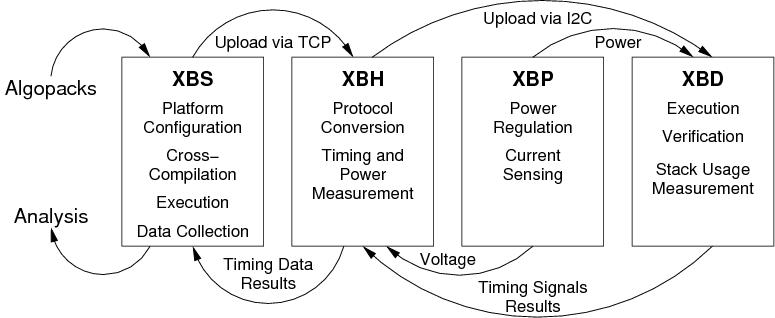
\includegraphics[scale=1.3]{../figures/xxbx_block}
        \end{center} 
        \begin{itemize}
          \item XXBX benchmarking System -- XBS 
          \begin{itemize}
            \item Software written in Python and runs on Linux.
            \item Cross-compiles cryptographic algorithms from SUPERCOP.
            \item Orchestrates benchmarking flow.
            \item Collects results and stores them into SQLite database.
          \end{itemize}
          \item XXBX Harness -- XBH 
          \begin{itemize}
            \item Passes applications, test data, and instructions to XBD.
            \item Measures timing and power consumption.
          \end{itemize}
          \item XXBX Power Shim -- XBP
          \begin{itemize}
            \item Senses and amplifies power consumption.
          \end{itemize}
          \item XXBX Device Under Test -- XBD
          \begin{itemize}
            \item Bootloader accepts commands and waits for application.
            \item Executes application with cryptographic algorithms.
          \end{itemize}
        \end{itemize}
      \end{block}
     
% ---------------------------------------------------------------------------
      \begin{block}{Benchmarking Flow}
        \begin{center}
          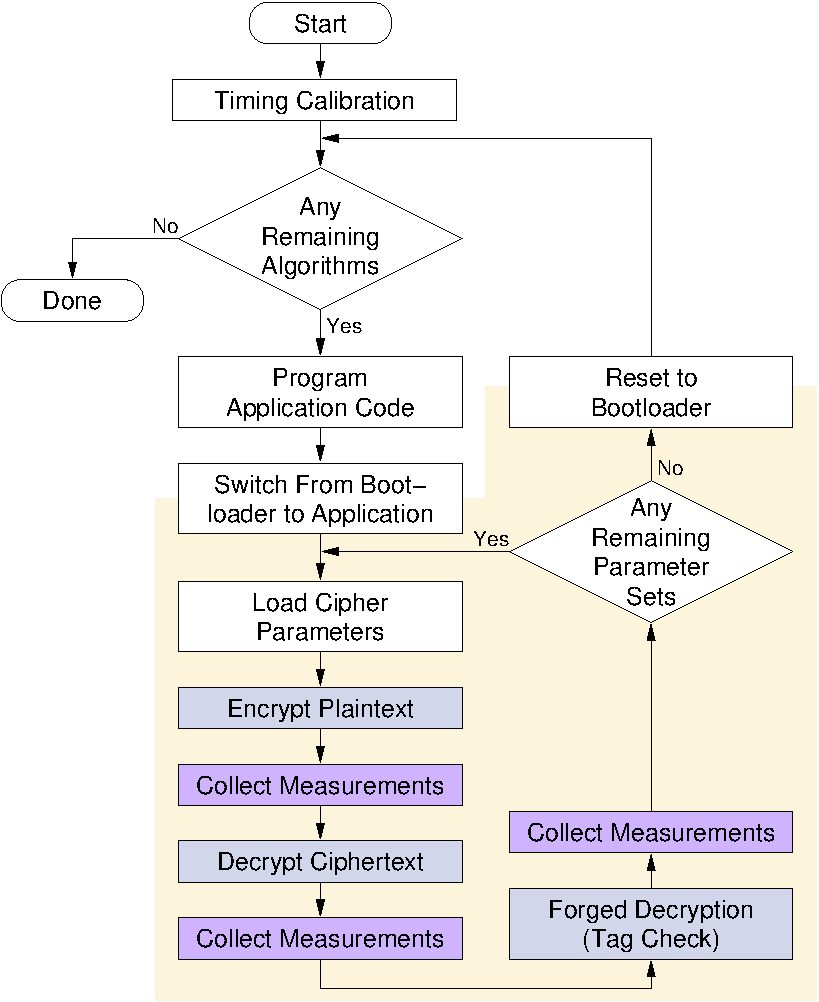
\includegraphics[scale=1.208]{../figures/xxbx_flow}
        \end{center} 
%          \begin{center}
%            \begin{minipage}{0.9\linewidth}
%            \setbeamercolor{padding}{fg=white, bg=cergbg3}
%            \begin{beamercolorbox}[rounded=true]{padding}%
%               \footnotesize%
%              \begin{lstlisting}
%[hardware]
%platform = msp430fr5994_16mhz
%[algorithm]
%operation = crypto_aead
%primitives =  0cipher
%              aes128n12t8silcv3
%[implementation]
%whitelist =  0cipher/empty
%             aes128n12t8silcv3/ref
%              \end{lstlisting}
%            \end{beamercolorbox}
%            \end{minipage}%
%          \end{center}
      \end{block}
     
% ---------------------------------------------------------------------------
      \begin{block}{RAM and ROM Usage Measurement}
        \begin{itemize}
          \item ROM Usage
            \begin{itemize}
              \item UNIX size command is run on generated application which
                    reports sizes of executable sections: \texttt{.bss}, .\texttt{data}, and \texttt{.text}.
              \item The sum of the \texttt{.text} and \texttt{.data} sections is the amount of ROM that is used.
            \end{itemize}
          \item RAM Usage
            \begin{itemize}
              \item Application paints memory with canary values.
              \item After execution of cipher operation, application checks
                    the number of addresses not containing canary values.
              \item This is the amount of stack memory used.
              \item The sum of the stack usage, \texttt{.data} section, and \texttt{.bss} section is the amount of RAM that is used.
            \end{itemize}
          
        \end{itemize}

      \end{block}

% ---------------------------------------------------------------------------
      \begin{block}{Timing Measurements}
        \begin{itemize}
          \item 16-bit timer TC to capture timing flag from XBD.
          \item Need additional timer TW at same rate to get interrupts when timer 
                wraps around.
          \item Higher priority TW counts wraps (w).
          \item TW can interrupt processing of TC ISR!
          \item Maximum time (t) is 35.8\,seconds (64-bit value) at 120\,MHz.
        \end{itemize}
        \begin{center}
          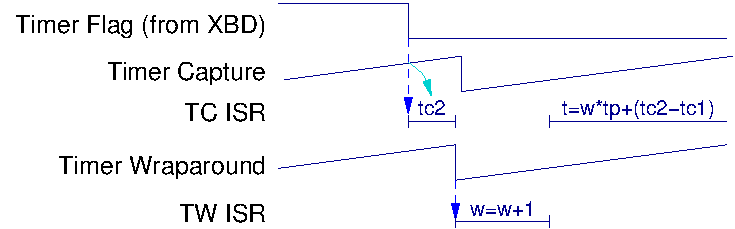
\includegraphics[scale=1.4]{./figures/timing}
        \end{center}
      \end{block}
	 
% ---------------------------------------------------------------------------
          
% ---------------------------------------------------------------------------
    \end{column}
% ---------------------------------------------------------------------------
%   THIRD COLUMN
% ---------------------------------------------------------------------------
   \begin{column}{.473\linewidth}
    
% ---------------------------------------------------------------------------
       \begin{block}{Power Measurement}
        \begin{minipage}{0.45\linewidth}
		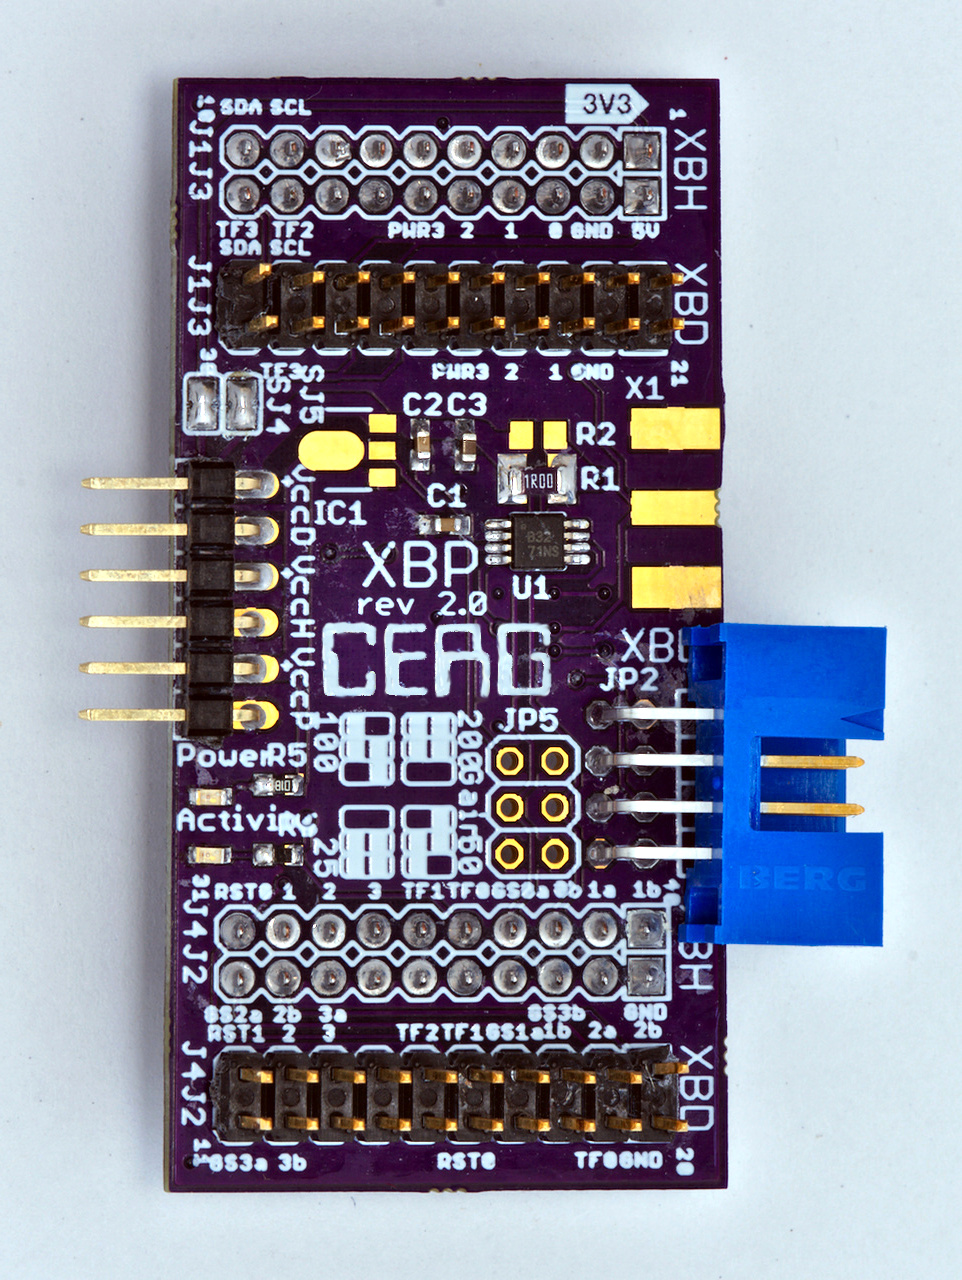
\includegraphics[scale=1.2]{../figures/xbp-full-top90}
        \end{minipage}%
%	\hspace{-5ex}
	\begin{minipage}{0.48\linewidth}
          \begin{itemize}
            \item Fits between XBH and XBD
            \item Contains I$^2$C pull-ups
            \item Space for power regulator
            \item Supports XBDs with 1.2\,V--5\,V
            %\item Eagle files in git
          \end{itemize}
          \begin{center}
            \vspace{-2ex}
            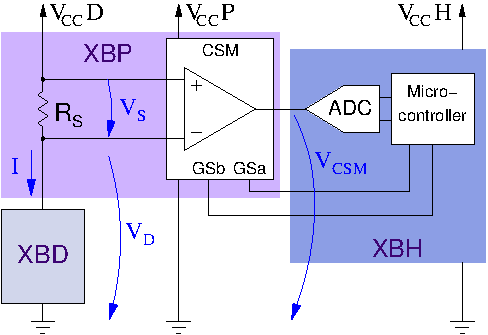
\includegraphics[scale=1.45]{../figures/ina225}
          \end{center} 
	\end{minipage} 
       \end{block}
% ---------------------------------------------------------------------------
       \begin{block}{CAESAR}
        \begin{itemize}
          \item Competition for Authenticated Encryption: Security, Applicability and Robustness
          \item Announced in 2013, finalists announced in March 2018.
          \item Round 3 had 16 algorithms with several variations.
          \item We benchmark them all on the microcontrollers supported by XXBX.
        \end{itemize}
       \end{block}

% ---------------------------------------------------------------------------
       \begin{block}{CAESAR Results}
        \begin{center}
        { \small%
          \renewcommand\tabcolsep{4pt}% 
          \rowcolors{3}{RoyalBlue!5}{RoyalBlue!20}%
          \begin{tabular}{|r||c|c|c|c||c|c}\hline
            \rowcolor{RoyalBlue!20}%
              & \multicolumn{4}{>{\columncolor{RoyalBlue!20}}c||}{\textbf{SASEBO}} 
              & \multicolumn{2}{>{\columncolor{RoyalBlue!20}}c}{\textbf{SAKURA}}      \\ 
            \rowcolor{RoyalBlue!20}%
            \rb{\textbf{Board}}   &          & \textbf{G} & \textbf{GII}  & \textbf{B}   & \textbf{X}   & \textbf{G}    \\ \hline
            \textbf{Control}      & Virtex-2 & Virtex-2   &               &              &              &               \\
            \rowcolor{RoyalBlue!5}%
            \textbf{FPGA}         & Pro      & Pro        &\rb{Spartan-3A}&\rb{Stratix-2}&\rb{Spartan-6}&\rb{Spartan-6} \\
            \rowcolor{RoyalBlue!20}%
            \textbf{DUT}          & Virtex-2 & Virtex-2   &               &              &              &               \\
            \textbf{FPGA}         & Pro      & Pro        &\rb{Virtex-5}  &\rb{Stratix-2}&\rb{Kintex-7} &\rb{Spartan-6} \\ 
            \textbf{Techn.}       
              & \multicolumn{1}{>{\columncolor{RoyalBlue!5}}r|}{130\,nm}  
              & \multicolumn{1}{>{\columncolor{RoyalBlue!5}}r|}{130\,nm}  
              & \multicolumn{1}{>{\columncolor{RoyalBlue!5}}r|}{65\,nm}        
              & \multicolumn{1}{>{\columncolor{RoyalBlue!5}}r||}{90\,nm}       
              & \multicolumn{1}{>{\columncolor{RoyalBlue!5}}r|}{28\,nm}    
              & \multicolumn{1}{>{\columncolor{RoyalBlue!5}}r}{45\,nm} \\       
                                  &          & RS232,     &               & RS232,       &              &               \\
            \rowcolor{RoyalBlue!20}%
            \rb{\textbf{PC Data}} &RS232     &FT245RL     &\rb{FT2232D}   & FT245RL      & USB          & USB           \\ 
            \rb{\textbf{Comms.}}  &          &(USB)       &\rb{(USB)}     & (USB)        &              &               \\ 
                                  &Discon-   &Discon-     &Discon-        &              &              &               \\ 
            \rowcolor{RoyalBlue!5}%
            \rb{\textbf{Status}}  &tinued    &tinued      &tinued         &              &              &               \\ \hline
          \end{tabular}
        }
        \end{center}
       \end{block}
% ---------------------------------------------------------------------------
       \begin{block}{Results of CAESAR Candidates}
        \vspace{-1ex}
         \begin{center}
           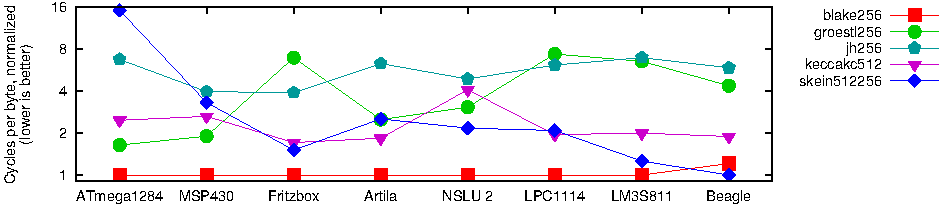
\includegraphics[width=0.9\linewidth]{../figures/cycles_per_byte}

           \vspace{-1ex}{\small Throughput}\vspace{1ex}

           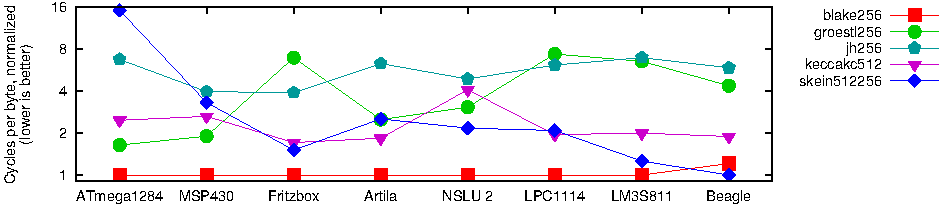
\includegraphics[width=0.9\linewidth]{../figures/cycles_per_byte}

           \vspace{-1ex}{\small RAM Usage}\vspace{1ex}

           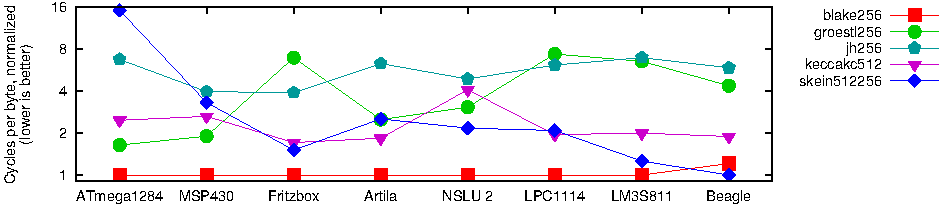
\includegraphics[width=0.9\linewidth]{../figures/cycles_per_byte}

           \vspace{-1ex}{\small ROM Usage}\vspace{1ex}

           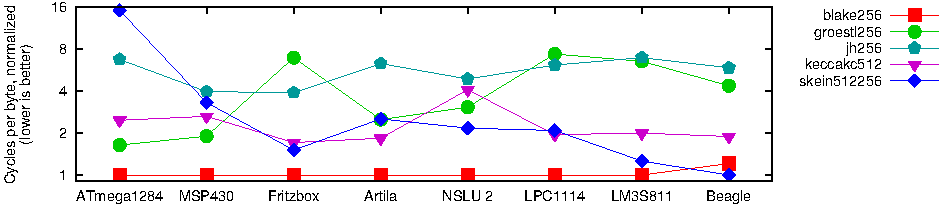
\includegraphics[width=0.9\linewidth]{../figures/cycles_per_byte}

           \vspace{-1ex}{\small Energy Consumption}
         \end{center}
       \end{block}

% ---------------------------------------------------------------------------
       \begin{block}{Future Research}
        \begin{itemize}
          \item Adapt XXBX to support Post Quantum Crytpography
          \item NIST is starting a Lightweight Cryptography Standardization Process for
                AEAD functions and Hash functions. The draft submission requirements 
                were published in April 2018. XXBX will support this effort.
          \item Expanding to other microcontrollers incl. 8-bit.
          \item Combine with FOBOS to allow side-channel leakage evaluation.
        \end{itemize}
       \end{block}

% ---------------------------------------------------------------------------
% ---------------------------------------------------------------------------
%      \begin{block}{References}
%        \footnotesize
%          \bibliographystyle{IEEEtran}
%          \bibliography{keccak}
%        %\input{keccakbib}
%      \end{block} 
   \end{column}
   \end{columns}

% ---------------------------------------------------------------------------
   \begin{columns}%[t]
   \begin{column}{0.977\linewidth}
      \begin{block}{Supported XBDs}
        \begin{minipage}{0.83\linewidth}
          \centering\renewcommand\tabcolsep{10pt}% 
          \rowcolors{2}{RoyalBlue!5}{RoyalBlue!20}%
    \begin{tabular}{l|c|ll|rrc|rr|r}
    \textbf{Board}   & \textbf{Manuf.}&\textbf{CPU}&\textbf{ISA}&\textbf{Bus}&\thb{f}&\textbf{HW}&\textbf{ROM}&\textbf{RAM} \\ \hline
%    Homemade         & Atmel     & ATmega1284P    &  AVR        &  8-bit &  20\,MHz &     &     &        \\
    MSP-EXP430F5529  & TI        & MSP430F        &  MSP430X    & 16-bit &  25\,MHz &     &   12kB &  10kB  \\
    MSP-EXP430FR5994 & TI        & MSP430FR       &  MSP430X    & 16-bit &  16\,MHz & AES &  256kB &   8kB  \\
    MSP-EXP432P401R  & TI        & ARM Cortex M4F &  ARMv7E-M   & 32-bit &  48\,MHz & AES &  256kB &  64kB  \\
    EK-TM4C123GXL    & TI        & ARM Cortex M4F &  ARMv7E-M   & 32-bit &  80\,MHz &     &  256kB &  32kB  \\ 
    EK-TM4C129EXL    & TI        & ARM Cortex M4F &  ARMv7E-M   & 32-bit & 120\,MHz & AES & 1024kB & 256kB  \\ 
    NUCLEO-F091RC    & STM       & ARM Cortex M0  &  ARMv6-M    & 32-bit &  48\,MHz &     &  256kB &  32kB  \\
    NUCLEO-F103RB    & STM       & ARM Cortex M3  &  ARMv7-M    & 32-bit &  72\,MHz &     &  128kB &  20kB  \\
%    chipKIT uC32     & Microchip & PIC32MX3xx     &  MIPS32 M4K & 32-bit &  80\,MHz &     &     &     &   \\
    \end{tabular}
        \end{minipage}
        \begin{minipage}{0.15\linewidth}
		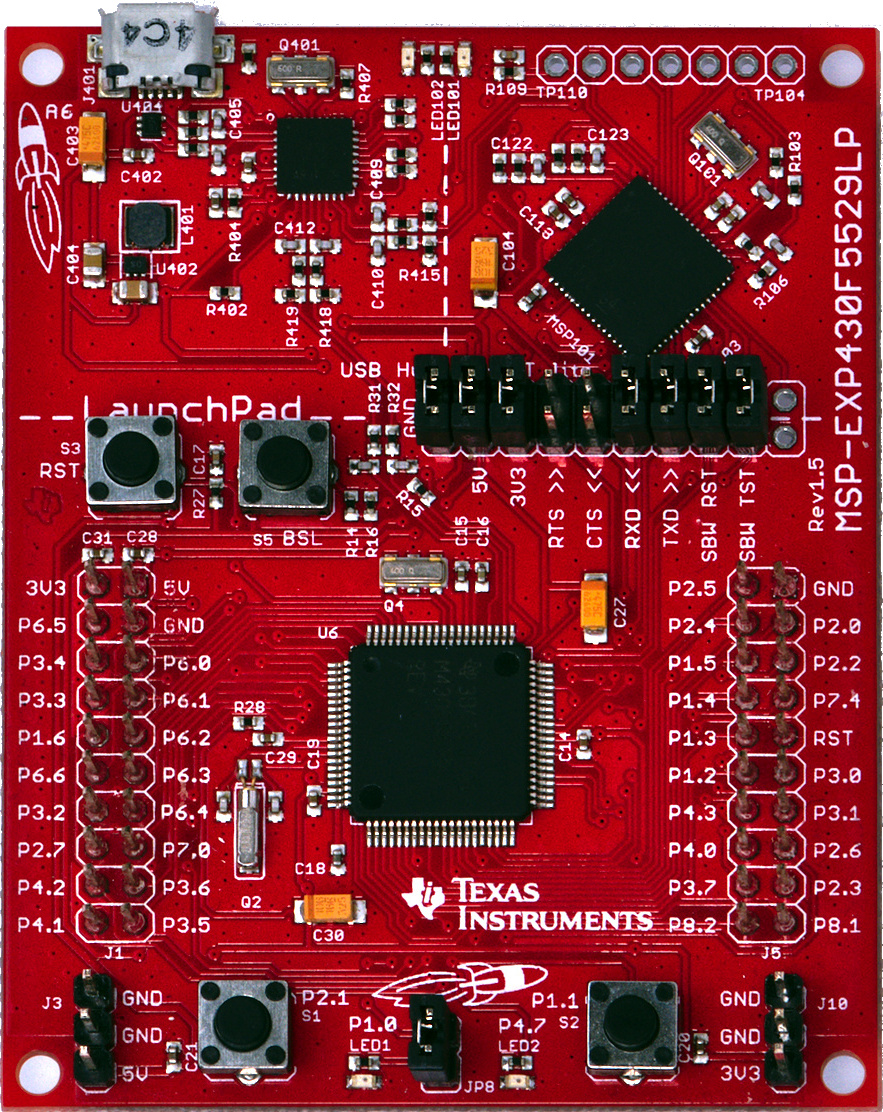
\includegraphics[scale=0.9]{../figures/msp-exp430f5529lp}
        \end{minipage}%
       \end{block}
\end{column}
\end{columns}
     
\end{column}
\end{columns}

\end{frame}
\end{document}

 
